\section{Proposed system}



\subsection{Security measures}

There are a number of slightly unique or novel security measures in the proposed system design. The following section attempts to explain how they work and the justification behind them.

\subsubsection{Customer support verification}

One common attack vector for bank customers is impersonating a member of customer support. Similarly, a member of customer support could potentially “go rogue” and attack a customer’s account.

While many consider phonelines to be a safe method of communication, “vishing” or “voice phishing” is on the rise. \cite{bbcPhone} \cite{bbcSmishing} Phone number spoofing can make an illegitimate call appear to be from a legitimate source. Holding open a line\footnote{
    During a landline phone call, depending on the network’s configuration, a line may be kept open after a receiver has hung up. For a short window of time, future calls they make will reuse the same line to the original caller. \cite{conArtists}
} can redirect a call from a customer to their bank towards an attacker.

Such techniques mean that verification of both Wondough Bank’s staff members and customers is necessary in every situation. The proposed system to satisfy such a goal is displayed in figure \ref{customerSupport}.

\begin{figure}
    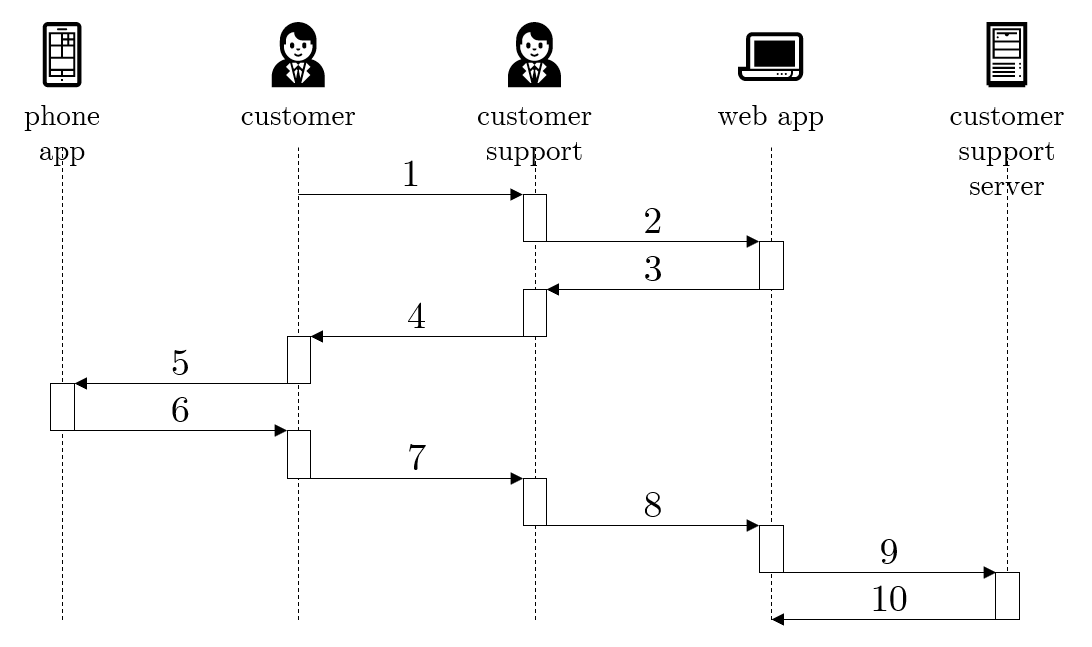
\includegraphics[width=\columnwidth]{images/customer-support}
    \caption{customer support verification}
    \centering
    \label{customerSupport}
\end{figure}

First, a customer contacts a member of customer support through a potentially insecure connection, such as a phone call. Alternatively, a member of customer support may contact the customer first. (step 1 on diagram)

To authenticate to the customer, the staff member’s customer service terminal will provide a one-time access code (OTAC) generated from the time, the staff member’s credentials, and the customer’s credentials. The staff member passes this to a customer, who verifies it using the Wondough Bank phone app. (steps 2-5 on diagram)

After verifying the customer support member’s OTAC, the phone app will provide a customer’s own OTAC. They must then provide this to the customer support representative. (step 6-8)

The customer service web application will send both OTACs to the customer support server, which will verify the codes server-side, before granting the staff member access to the customer’s account.

Such a system requires authorisation and consent from both the staff member and the customer before any changes to a customer’s account may be made.

\subsubsection{Merchant authorisation}

Preventing a third party impersonating a merchanting is a similarly high priority requirement.  The proposed method for a merchant billing a customer’s account is shown in Figure \ref{merchantBilling}.

\begin{figure}
    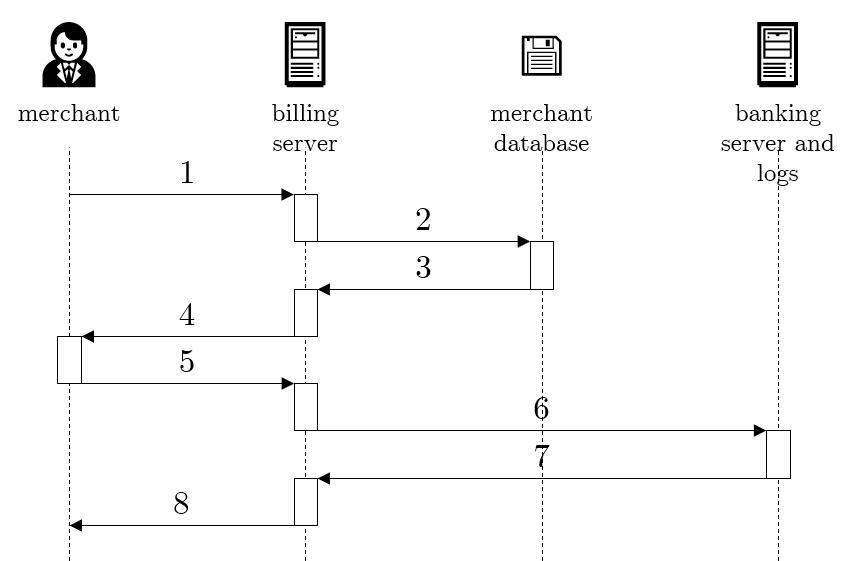
\includegraphics[width=\columnwidth]{images/merchant-billing}
    \caption{merchant billing customer’s account}
    \centering
    \label{merchantBilling}
\end{figure}

To be accepted as a merchant, a third party must go through a verification process , during which they will be assigned a secret key, and an identifying name (IN). Since every merchant is assigned a unique secret key, damage if one such key is discovered is mitigated.

Upon connecting to the billing server, a merchant will supply their IN, a timestamp for the transaction, and a hash of their message encrypted with their secret key (message authentication code, MAC). The timestamp will prevent a replay attack from being performed, while the MAC will prevent an attacker simply changing the timestamp. (step 1)

When receiving their initial communication, the billing server will reference the merchant database for a secret key matching the IN provided. If one is not found, the whole communication is rejected. Otherwise, it is used to decrypt the MAC and verify the integrity and origin \footnote{
    While MACs do not normally provide non-repudiation in this way, each secret key is unique to a single merchant, and thus may be used to identify one. 
} of the message. (step 2, 3)

Future traffic sent across the network is encrypted with the merchant’s secret key, providing secrecy. The billing server responds to the merchant, accepting the request, and the merchant replies with a billing for a customer. (step 4, 5) The transaction is sent to the banking server, and the communication is logged. (step 6)

If the whole process is successful, the banking server will reply to the billing server that the transaction was successful, which will forward the message to the merchant. (step 7, 8)

\subsection{Threat model}

There are a wide variety of possible attacks upon the proposed Wondough bank system. The STRIDE system was used to provide a threat model.

\subsubsection{Spoofing}

\begin{enumerate}
    \item Impersonate audit
    \begin{enumerate}
        \item Gain access to logs
        \begin{enumerate}
            \item Retrieve potentially valuable security information
            \begin{enumerate}
                \item Pinpoint system failures to find new vulnerabilities
                \item Find support tickets to impersonate customer support for other attacks
            \end{enumerate}

            \item Reconstruct customer’s bank information from transaction history
            \begin{enumerate}
                \item Transactions
                \item Detail changes (address, phone number, etc..)
            \end{enumerate}
        \end{enumerate}
    \end{enumerate}
    
    \item Impersonate customer support.
    \begin{enumerate}
        \item Gain access to a customer's account
        \item Change a customer's details
        \item Access a customer's details to commit identity fraud
        \item Convince a customer to move money out of their account
    \end{enumerate}

    \item Impersonate a merchant
    \begin{enumerate}
        \item Bill customers incorrectly
    \end{enumerate}

    \item Impersonate IT in any trust boundary
    \begin{enumerate}
        \item May provide direct access to servers or databases
    \end{enumerate}

    \item Impersonate the webserver or the support server
    \begin{enumerate}
        \item Genuine users could connect to them mistakenly, allowing credentials to be stolen
        \item Could forge requests to other servers
    \end{enumerate}
\end{enumerate}

\subsubsection{Tampering}

\begin{enumerate}[resume]
    \item IT could change logs without permission
    \begin{enumerate}
        \item Hide other actions in system
    \end{enumerate}

    \item IT could change account database without permission
    \begin{enumerate}
        \item Move money without permission
        \item Change customer details
    \end{enumerate}

    \item IT could change merchant database without permission
    \begin{enumerate}
        \item Allow arbitrary authorisation of merchants
        \item Allow arbitrary de-authorisation of merchants
    \end{enumerate}

    \item IT could alter support tickets
    \begin{enumerate}
        \item Create fake tickets to waste staff time
        \item Alter/delete tickets to cause customer dis-satisfaction
    \end{enumerate}
\end{enumerate}

\subsubsection{Repudiation}

\begin{enumerate}[resume]
    \item The customer pretends to be the victim of fraud
    \begin{enumerate}
        \item The bank must cover assets lost by fraud
    \end{enumerate}

    \item Malicious activity by IT staff
    \item Malicious activity by customer support
\end{enumerate}

\subsubsection{Information disclosure}

\begin{enumerate}[resume]
    \item Malicious access to a customer's account by member of customer support

    \item Malicious access to a customer's account by member of IT
    \begin{enumerate}
        \item Alter previous transactions
        \item Create new transactions
        \item Steal information
    \end{enumerate}

    \item A member of IT successfully attacks the account database, revealing a customer's information

    \item A member of IT accesses any of the keys used for encryption
\end{enumerate}

\subsubsection{Denial of service}

\begin{enumerate}[resume]
    \item DoS attack on website
    \item DoS attack on customer support service
    \item DoS attack on billing server
    \item DoS attack on banking server
    \item DoS attack on logs
\end{enumerate}

\subsubsection{Elevation of privilege}

\begin{enumerate}[resume]
    \item XSS attack using website
    \item SQL Injection using website registration form
    \item XSS attack or SQL injection using customer support software
    \item Different servers could validate data differently when sending data to be logged – if some paths give different results, an attacker could exploit this
    \item An attacker could bypass client-side validation and send un-validated information to a server
\end{enumerate}

\subsection{Threat solution and evaluation}



\subsection{Legal and economic considerations}

There are a number of other considerations which must be considered for the design of the Wondough banking system. While legal requirements are perhaps the most obvious, and regulations are effectively mandatory, economic constraints on the system must also be considered.

\subsubsection{Legal requirements}



\subsubsection{Economic constraints}

A system which fully meets or exceeds all requirements may still be prohibitively expensive for a small scale, start-up company like Wondough Bank to deploy, and thus may be unrealistic. It is necessary to consider the compromises which have to be made when designing such a system. 

\subsubsubsection{Hosting}

Firstly, the choice of server host is important. While larger banks are able to afford their own dedicated servers for online banking, it may be necessary for a company on the scale of Wondough Bank to turn to a cloud-based hosting service such as Amazon Web Services or Microsoft Azure. While an in-house hosting solution may be cheaper in the long run, an organisation such as Wondough Bank may be unable to meet the necessary up-front expenditure.

However, hosting Wondough Bank's web-app in the cloud has some key advantages. Firstly, while the organisation is currently small, their intended scope for expansion is large. This is an area in which cloud services excel, and Wondough would need only to pay for any increased usage. If Wondough Bank were to install their own hosting infrastructure, they may find future expansion or upgrades costly.

Also, many hosts are willing to accept a large part of the responsibility for the security of data transmitted and stored on their servers. This means that Wondough Bank's resources may be focused more in other areas, and allows them to transfer risk to third parties. However, this may be disadvantageous, and Wondough Bank may want to be certain exactly what level of security data is afforded - a task which could be difficult when dealing with a large hosting company.

\subsubsubsection{Key security}

In the interests of security, Hardware Security Modules (HSMs) would be advantageous for any implementation of a secure system. Fortunately, many hosting services provide support for storing keys and passwords on HSMs.

\subsubsubsection{Software}

For an organisation such as Wondough Bank, software lisences may be expensive. For example, certain implementations of SQL can be highly-priced. However, similarly to HSMs, hosting services may offer a "pay-by-use" pricing system for such software, moving a single fixed cost to several smaller, variable ones.